\documentclass{report}
\usepackage{amsthm}
\usepackage{comment}
\usepackage{mathbbol}

\theoremstyle{definition}
\newtheorem{definition}{Definition}
\usepackage[skip=4pt]{caption}
\usepackage{graphicx}
\usepackage{xcolor}
\usepackage{hyperref}
\usepackage{graphicx}
\usepackage{float}
\usepackage{amsmath}
\usepackage{relsize}
\usepackage{listings}
\usepackage{enumitem}
\usepackage{fancyhdr}
\usepackage{booktabs}
\usepackage{multirow}
\usepackage{tabularx}
\usepackage{multirow}
\colorlet{lightgrey}{lightgray}
\usepackage{colortbl}
\usepackage[bibstyle=authoryear, style=numeric, citestyle=numeric-comp, backend=bibtex]{biblatex}
\bibliography{bibliography/krr,bibliography/procs,local}

% Begin Variables definition
\newcommand\widthimg{12cm}

\lstdefinestyle{mystyle}{
    basicstyle=\ttfamily,
    % frame=single,
    breaklines,
    columns=fullflexible,
    breakindent=1.2em,
    breakatwhitespace,
    numbers=left, 
    escapechar=|
}

\DeclareCaptionType{equ}[][]

% End Variables definition





\title{%
\Huge{Conflict-based Plan Merging for Multi-agent Pathfinding}\\[0.2cm]
\Large{Master Thesis}
}
\author{
\\[1.5cm] \LARGE{Aurélien SIMON}
\\[0.2cm] \small{Matrikel-Nr: 806567 }
\\[1cm] \textbf{Supervisors}
\\[0.2cm] Klaus Strauch 
\\[0.2cm] Etienne Tignon
\\[0.2cm] Torsten Schaub
\\[2cm] \Large{Potsdam University}
\\[0.4cm] Master Cognitive Systems: Language, Learning and Reasoning 
\\[1cm]
}


\begin{document}
\pagestyle{fancy}

\maketitle

\pagenumbering{arabic} 

\fancyhead{} % clear all header fields
% \fancyfoot{} % clear all header fields

% \fancyfoot{} % clear all footer fields
\fancyhead[L]{Aurélien Simon}
\fancyhead[R]{Potsdam University}

\newpage

\begin{abstract}
    
     Multi-Agent Pathfinding (MAPF) is an artificial intelligence problem with wide-ranging applications including GPS, video games, and traffic control. MAPF involves orchestrating multiple agents to navigate from initial positions to specific destinations while avoiding collisions. In this work, we introduce a "Plan Merging" approach, a three-step approach based on path conflicts designed to tackle MAPF problems. The three steps are designated Individual Path Finding, Path Selection and Solving. We show that in certain cases, our proposed approaches can outperform classical MAPF methods. However, it also highlights the inherent limitations of our Plan Merging techniques, particularly in scenarios where obtaining a complete solution is challenging or not feasible.
    \\[1cm]
    \indent Multi-Agent Pathfinding (MAPF) ist ein Problem der künstlichen Intelligenz mit weitreichenden Anwendungen wie GPS, Videospiele und Verkehrskontrolle. Bei MAPF geht es darum, mehrere Agenten so zu koordinieren, dass sie von ihren Ausgangspositionen zu bestimmten Zielen navigieren und dabei Kollisionen vermeiden. In dieser Arbeit stellen wir einen "Plan Merging"-Ansatz vor, einen dreistufigen Ansatz, der auf Pfadkonflikten basiert und zur Lösung von MAPF-Problemen entwickelt wurde. Die drei Schritte werden als Individual Path Finding, Path Selection und Solving bezeichnet. Wir zeigen, dass die von uns vorgeschlagenen Ansätze in bestimmten Fällen die klassischen MAPF-Methoden übertreffen können. Es werden jedoch auch die inhärenten Grenzen unserer Techniken zur Zusammenführung von Plänen hervorgehoben, insbesondere in Szenarien, in denen der Erhalt einer vollständigen Lösung schwierig oder nicht möglich ist.

\end{abstract}

\newpage

\indent \textbf{Declaration of originality} \\
\noindent I confirm that the master's thesis I have submitted is my own original work. I have not utilized any external sources or aids except for the ones explicitly mentioned. In cases where I have incorporated verbatim passages from other works, I have duly acknowledged the source through proper citations. This work has not been previously submitted for any course or examination, nor has it been presented to any other authority for approval. \\[1cm]

\indent \textbf{Eigenständigkeitserklärung} \\
\noindent Ich versichere, dass ich die eingereichte Masterarbeit selbstständig verfasst habe. Ich habe keine externen Quellen oder Hilfsmittel verwendet, außer denen, die ausdrücklich genannt sind. In den Fällen, in denen ich wörtliche Passagen aus anderen Arbeiten übernommen habe, habe ich die Quelle durch ordnungsgemäße Zitate ordnungsgemäß angegeben. Diese Arbeit wurde weder für einen Kurs oder eine Prüfung eingereicht, noch wurde sie einer anderen Behörde zur Genehmigung vorgelegt. \\[2cm]



\indent Signature/Unterschrift \\[1.2cm]

\indent Place/Ort, Date/Datum

\newpage
\tableofcontents

\listoffigures

\lstlistoflistings
\newpage


% \setcounter{page}{1}
% \fancyfoot[R]{\thepage}





\chapter{Introduction \& Background}
\input{section/introduction.tex}
\section{Introduction \& Background}
\subsection{What is MAPF?}
\begin{frame}
    \textbf{What is Multi Agent PathFinding?} \\[1cm]

    \(\blacktriangleright \) Multi-Agent Pathfinding (MAPF) involves planning collision-free paths for multiple agents in a shared environment.

    \(\blacktriangleright \) Various application : warehouse management~\cite{wurman2008coordinating}, video games~\cite{ma2017feasibility}, routing, planning, robotics~\cite{veloso2015cobots}\dots


\end{frame}

\begin{frame}{An example}
    
    \begin{figure}[H]
        \centering
        \caption{Example of Multi agent Pathfinding}
        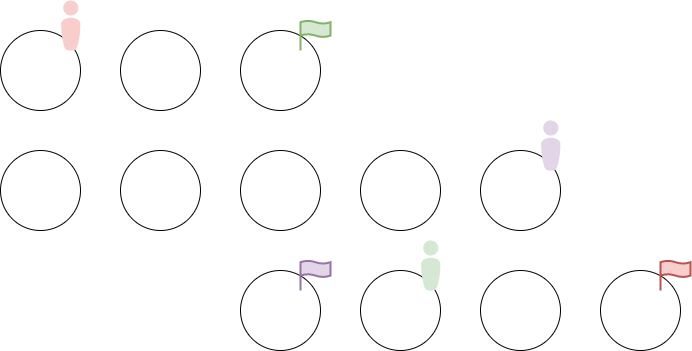
\includegraphics[width=\widthimg]{img/MAPF_example_1.drawio.png}
    \end{figure}

\end{frame}


\begin{frame}{An example}
    
    \begin{figure}[H]
        \centering
        \caption{Example of Multi agent Pathfinding}
        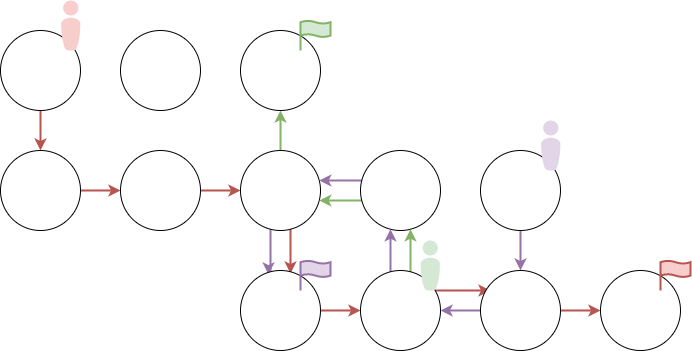
\includegraphics[width=\widthimg]{img/MAPF_example_2.drawio.png}
    \end{figure}

\end{frame}


\begin{frame}{Settings}
    MAPF is defined on a graph.
    
    \begin{block}{Nomenclature}
        \begin{itemize}
            \item The output is a plan \(\Pi\)
            \item \(\Pi\) is a collection of \(\pi\)
        \end{itemize}
    \end{block}
    
    
    \begin{figure}[H]
        \centering
        \caption{Considered conflicts}
        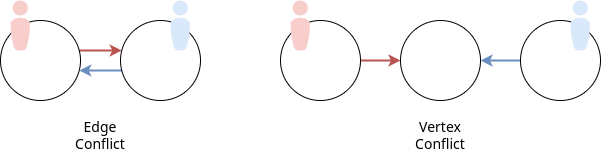
\includegraphics[width=\widthimg]{img/conflict_type.drawio.png}
    \end{figure}


\end{frame}



\subsection{Plan Merging: Motivation, Principle \& Overview}

\begin{frame}{Plan Merging: Motivation, Principle \& Overview}


    \textbf{Principle}
    \begin{itemize}
        \item From path(S) computed without considering conflict
        \item Try to find a conflict free plan out of the previously computed paths
    \end{itemize}


    \textbf{Motivation}
    \begin{itemize}
        \item Computing multiple individual path(s) is not expensive
        \item + Combining them is still faster 
    \end{itemize}


    \textbf{Overview}
    \begin{figure}[H]
        \centering
        \caption{Overview of the process}
        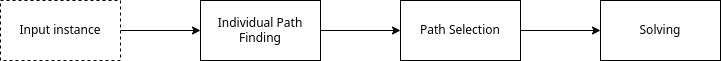
\includegraphics[width=\widthimg]{img/overview.drawio.png}
    \end{figure}
\end{frame}


\input{section/overview.tex}

\chapter{Individual Path Finding}
\section{Individual Path Finding}
\begin{frame}{Individual Path Finding}
    What is Individual Path finding?
    \begin{itemize}
        \item Creating \(n\) paths for each agents
        \item Creating \textbf{different kind of paths}
        \item Paths created do not consider collision with other paths
    \end{itemize}
    \begin{itemize}
        \item For each agent \(a\), we have \(\gamma_a\) = \(\{\pi_0,\dots,\pi_n\}\)
        \begin{itemize}
            \item \(\gamma\) is a set of paths
        \end{itemize}
        \item \(\tau\) representing the output of IPF 
        \begin{itemize}
            \item \(\tau = \{\gamma_a, \gamma_{a'}, ...\}\) is a set of set of paths
        \end{itemize}
    \end{itemize}
\end{frame}


\begin{frame}{IPF output example}
    \begin{figure}[H]
        \centering
        \caption{Example of a \(\tau = \{\gamma_r, \gamma_b, \gamma_g\}\)}\label{fig:ipf_example}
        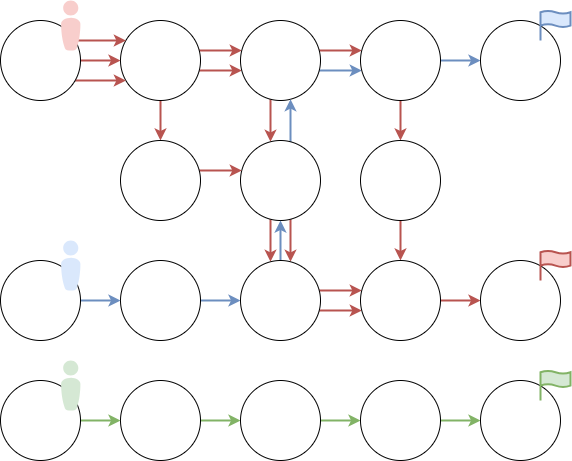
\includegraphics[width=7cm]{img/ipf_example.drawio.png}
    \end{figure}
\end{frame}



\subsection{IPF Computation}

\begin{frame}{Base IPF Computation}
    Principle of Base IPF computation
    \begin{figure}[H]
        \centering
        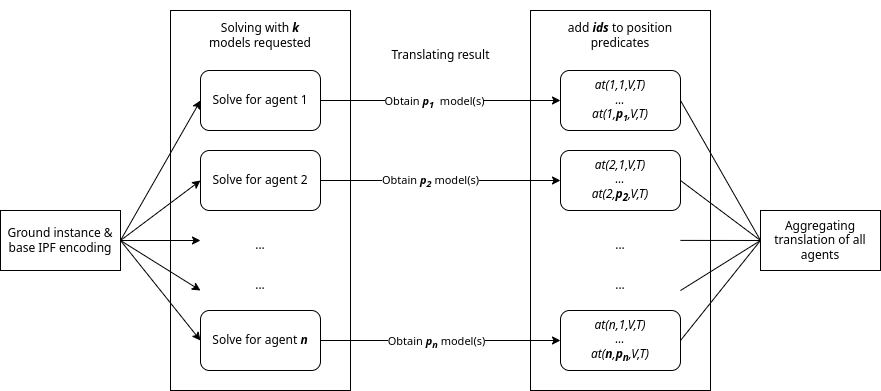
\includegraphics[width=11cm]{img/flowchart_ipf_computation.drawio.png}
    \end{figure}
\end{frame}


\chapter{Path Selection}
\section{Path Selection}
\begin{frame}{Path Selection}
    Path Selection aims to create an ``interesting'' subcomponent \(\tau'\) of \(\tau\). 

    \begin{figure}[H]
        \centering
        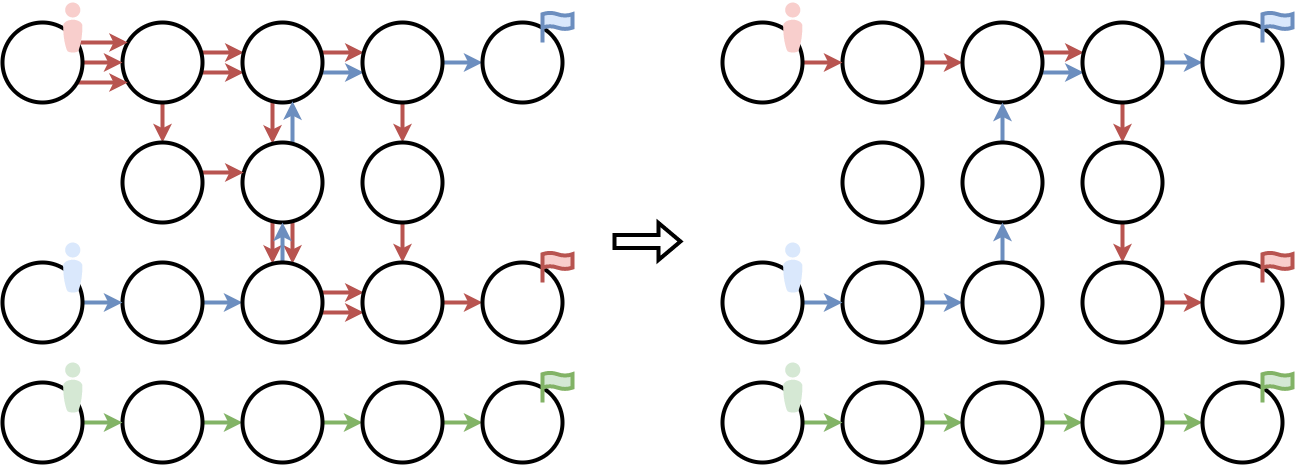
\includegraphics[width=11cm]{img/pm_example_intro.png}
    \end{figure}

\end{frame}


\subsection{Path Elimination}
\begin{frame}{Path Elimination}
    \textbf{  Path Elimination} is the process of the removing paths that exhibit potential issues. 
    
    \begin{block}{Why not find brute force a conflict-free set of paths directly?}
        \(\text{    }\blacktriangleright\) Slow with a lot of agents and paths, we need some preliminary process first
    \end{block}

    Two ways:
    \begin{itemize}
        \item \textbf{Based on heatmaps}
        \item Based on potential conflict
    \end{itemize}

\end{frame}


\subsection{Individual Heatmap}
\begin{frame}[fragile]{Individual Heatmap}
    Individual Heatmap is about projecting likelihood of presence of an agent on vertices
at each step.

    \[
        \phi(\gamma,v,t) = \frac{| \{\pi|\pi \in \gamma,\pi(t) = v\}|}{|\gamma|}
    \]


\end{frame}

\begin{frame}{Individual Heatmap example 1/5}

    \begin{figure}[H]
        \centering
        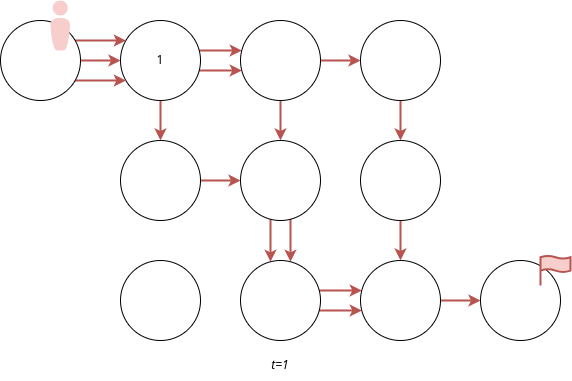
\includegraphics[width=9cm]{img/individual_heatmap_p1.drawio.png}
    \end{figure}
\end{frame}

\begin{frame}{Individual Heatmap example 2/5}
    \begin{figure}[H]
        \centering
        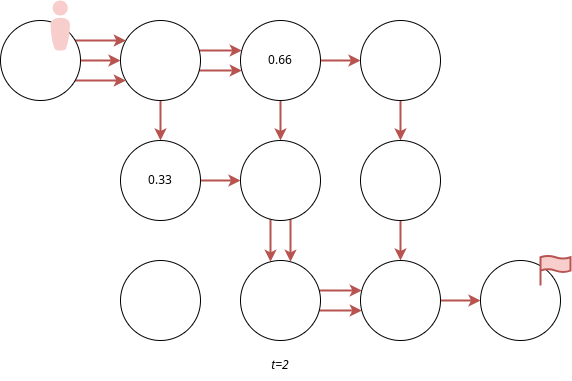
\includegraphics[width=9cm]{img/individual_heatmap_p2.drawio.png}
    \end{figure}
\end{frame}


\begin{frame}{Individual Heatmap example 3/5}
    \begin{figure}[H]
        \centering
        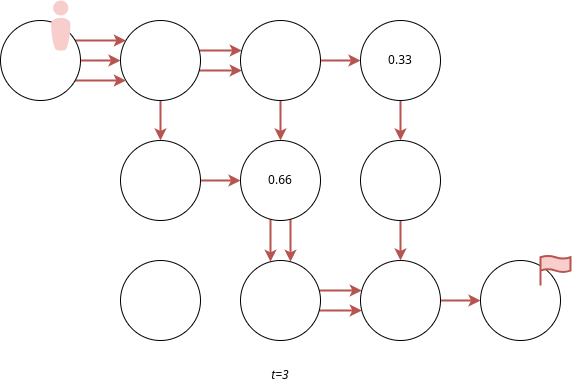
\includegraphics[width=9cm]{img/individual_heatmap_p3.drawio.png}
    \end{figure}
\end{frame}

\begin{frame}{Individual Heatmap example 4/5}
    \begin{figure}[H]
        \centering
        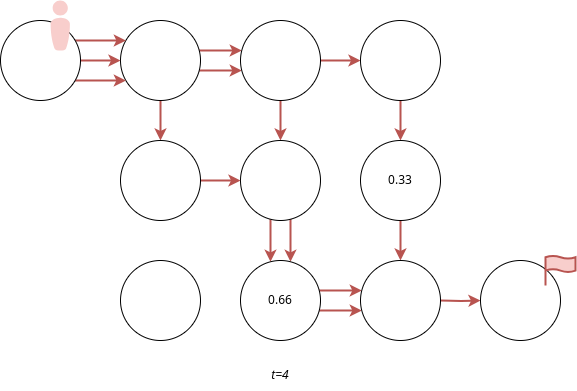
\includegraphics[width=9cm]{img/individual_heatmap_p4.drawio.png}
    \end{figure}
\end{frame}

\begin{frame}{Individual Heatmap example 5/5}
    \begin{figure}[H]
        \centering
        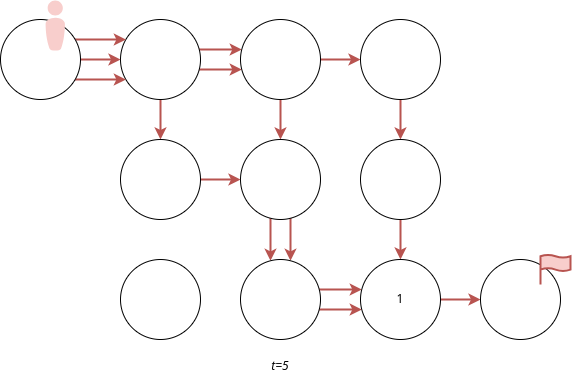
\includegraphics[width=9cm]{img/individual_heatmap_p5.drawio.png}
    \end{figure}
\end{frame}

\subsection{Global Heatmap}

\begin{frame}{Global Geatmap}
    We derive a \textbf{Global Heatmap} (GH) through the aggregation of all Individual Heatmaps
    \[
        \Phi(\tau,v,t) = \frac{ \sum_{\gamma \in \tau}\phi(\gamma,v,t)}{|\tau|}
    \]

    Global Heatmap do not represent a direct indicator of the likelihood of presence but instead an indicator of ``usage of vertices'' by multiple agents
\end{frame}


\begin{frame}{Global Heatmap example 1/5}
    \begin{figure}[H]
        \centering
        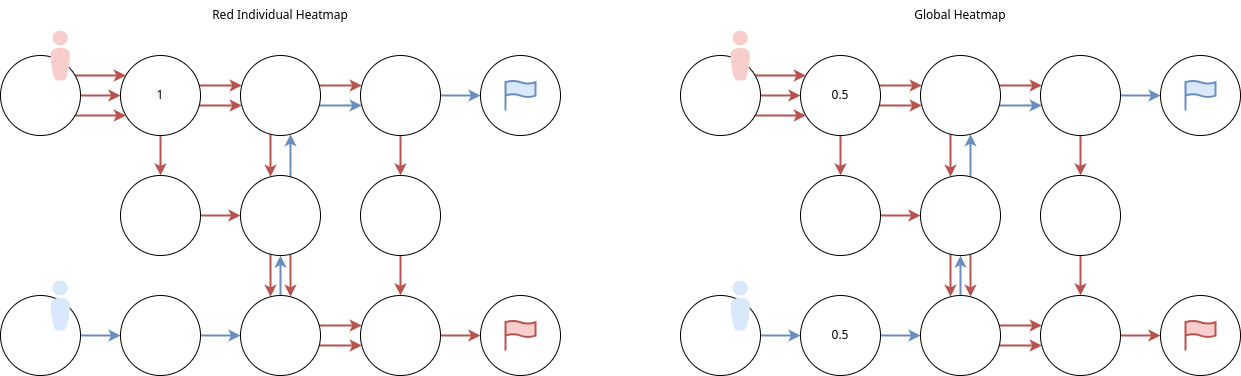
\includegraphics[width=11cm]{img/global_heatmap_p1.drawio.png}
    \end{figure}
\end{frame}


\begin{frame}{Global Heatmap example 2/5}
    \begin{figure}[H]
        \centering
        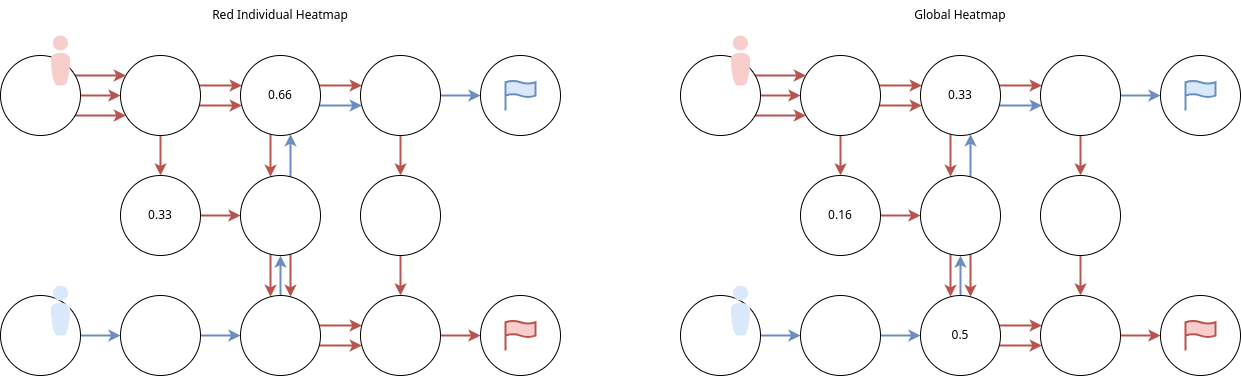
\includegraphics[width=11cm]{img/global_heatmap_p2.drawio.png}
    \end{figure}
\end{frame}



\begin{frame}{Global Heatmap example 3/5}
    \begin{figure}[H]
        \centering
        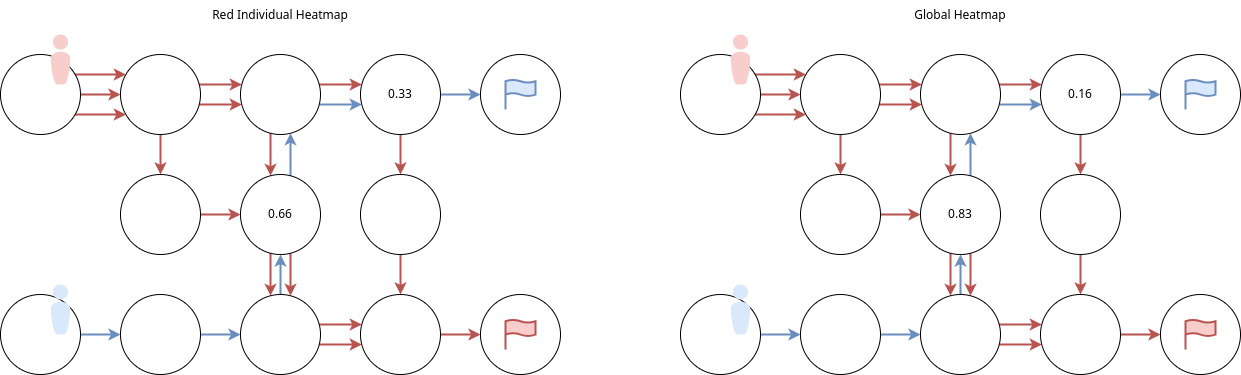
\includegraphics[width=11cm]{img/global_heatmap_p3.drawio.png}
    \end{figure}
\end{frame}


\begin{frame}{Global Heatmap example 4/5}
    \begin{figure}[H]
        \centering
        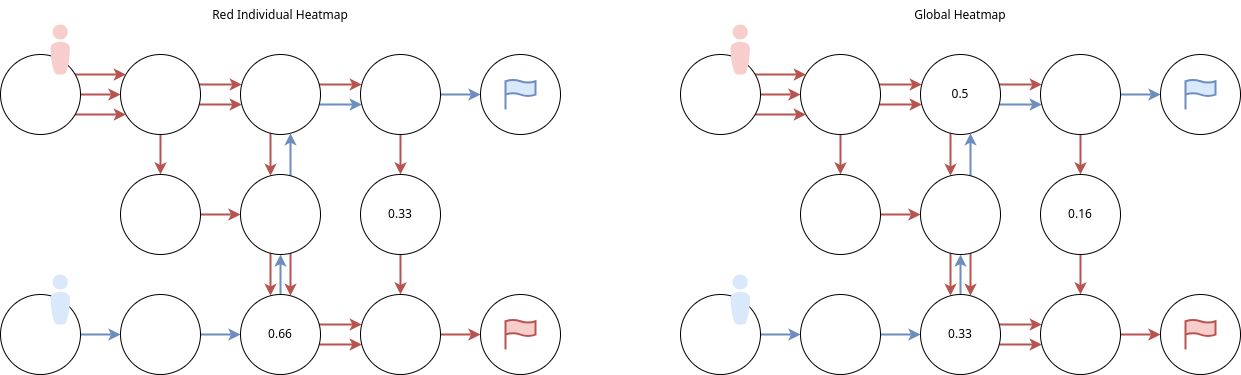
\includegraphics[width=11cm]{img/global_heatmap_p4.drawio.png}
    \end{figure}
\end{frame}


\begin{frame}{Global Heatmap example 5/5}
    \begin{figure}[H]
        \centering
        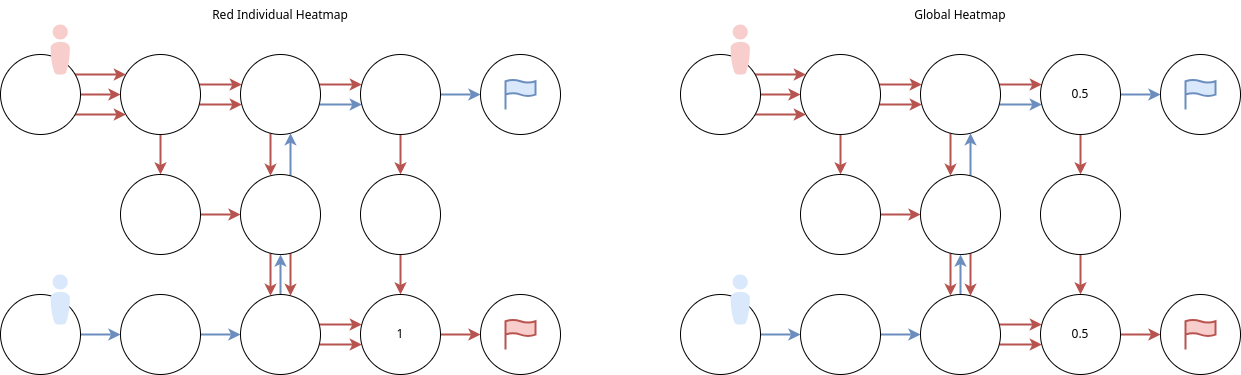
\includegraphics[width=11cm]{img/global_heatmap_p5.drawio.png}
    \end{figure}
\end{frame}



\begin{frame}{Path Elimination Approaches Summary}
    \textbf{Eliminate paths based on heatmaps:}

            \begin{itemize}
                \item \textbf{Unique Heatmap Values:}
                    \begin{itemize}
                        \item Order assignments by global heatmap values.
                        \item Identify critical vertices and eliminate paths containing them.
                    \end{itemize}
                \item \textbf{Threshold-based Elimination:}
                    \begin{itemize}
                        \item Define thresholds (\(\mathcal{H}\)) based on various properties.
                        \item A vertex is denoted critical if its global heatmap value is above the threshold
                    \end{itemize}
                \item \textbf{Sums of Global Heatmap Values:}
                    \begin{itemize}
                        \item For every path, we sum the value of each global heatmap value the paths goes on
                        \item We eliminate \(k\) paths based on the summed value 
                    \end{itemize}
            \end{itemize}
\end{frame}



\begin{frame}{An example}
    \begin{figure}[H]
        \centering
        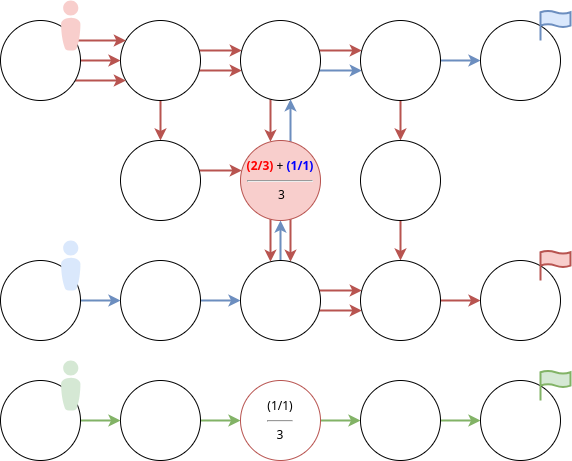
\includegraphics[width=\widthimg]{img/pe_one_heatmap_value_example.drawio.png}
    \end{figure}
\end{frame}





\subsection{Path Selection}
\begin{frame}{Path Selection: towards (partial) solving}
    In the end, what paths are we using? 


    \begin{itemize}
        \item Objective 1: Identify a conflict-free partial plan \(\hat{\Pi}\)
        \begin{itemize}
            \item At most one path per agent 
        \end{itemize}
        \item Objective 2: Create a subgraph 
        \begin{itemize}
            \item At least one path per agent
        \end{itemize}
    \end{itemize}
\end{frame}



\chapter{(Partial) Solving}
\input{section/partialsolving.tex}

\chapter{Benchmarks \& Conclusion}

\input{section/benchmarks.tex}
\section{Conclusion}
\begin{frame}{Conclusion}
\begin{itemize}
    \item Implemented a whole process for Plan merging
    \item Explored different ways of solving
    \item Defined a Plan Merging approach based on heatmaps as a selection process (which can be used for future work)
    \item We showed that some of the approaches we defined can outperform classical MAPF
\end{itemize}
\end{frame}


\begin{frame}{Thanks}
    
    \centering 
    Thank you for your attention !! :) \\[1cm] 
    
    Special thanks to Klaus Strauch, Etienne Tignon, Torsten Schaub \& Lydia Körber 

\end{frame}


\newpage


\section*{References}
\printbibliography[heading=none]

\input{section/appendix.tex}
\end{document}